\documentclass[runningheads]{llncs}

\usepackage[T1]{fontenc}
\usepackage{graphicx}
\usepackage{amsmath}
\usepackage{amssymb}
\usepackage{booktabs}
\usepackage{hyperref}
\usepackage{float}
\usepackage{multirow}
\usepackage{caption}
\usepackage{tikz}
\usepackage{array}
\usepackage{listings}
\usepackage[T1]{fontenc}
\usepackage{xurl}
\usepackage{seqsplit}
\usepackage{microtype}

\emergencystretch=3em
\sloppy

\begin{document}

\title{Formal modelling and verification of neuronal archetypes}

\author{Thi-Thuy-Duong Pham\inst{1} \and
Elisabetta De Maria\inst{1} \and
Robert De Simone\inst{2}}

\authorrunning{T.T.D Pham et al.}

\institute{I3S, CNRS, Université Côte d'Azur, Sophia Antipolis, France\\
\email{thi-thuy-duong.pham@etu.univ-cotedazur.fr}\\
\email{elisabetta.de-maria@univ-cotedazur.fr} \and
Centre Inria d'Université Côte d'Azur, Sophia Antipolis, France\\
\email{robert.de\_simone@inria.fr}}

\maketitle

\begin{abstract}
Spiking Neural Networks (SNNs) are considered to be more biologically realistic models of neural computation than traditional artificial neural networks, as they encode and process information through the timing of discrete spikes rather than continuous activation values. Within this framework, neuronal archetypes represent canonical connectivity patterns that serve as fundamental building blocks for constructing larger and more complex neural circuits. Understanding the dynamical properties of these archetypes is therefore a crucial first step toward explaining and predicting the behavior of the networks that emerge from their composition.

In this work, we propose a formal verification framework, implemented in the tool \texttt{snn\_mc}, for analyzing the dynamics of neuronal archetypes through model checking. Archetype structures and Leaky Integrate-and-Fire (LIF) neuron parameters are specified using a domain-specific language (DSL), automatically translated into discrete NuSMV models. Relevant dynamical properties are expressed in Computation Tree Logic (CTL) and Linear Temporal Logic (LTL) and verified exhaustively using the NuSMV model checker, which produces counterexample traces whenever a property is violated. Through representative archetype case studies, we demonstrate how this approach provides rigorous guarantees about archetype behavior and supports the systematic study of biologically inspired neural circuits. Finally, we discuss the extension of this framework toward the verification of archetype compositions, paving the way for the formal analysis of larger spiking neural networks built from these elementary structures.

\keywords{Spiking Neural Networks \and Neuronal Archetypes \and Biological Neural Networks \and Model Checking \and Dynamic Properties}
\end{abstract}

\section{Introduction}
% ---------------------------------------------------------------

Understanding the human brain remains one of the most profound challenges in science.
Biological neural networks exhibit highly complex dynamics that are difficult to
analyze through observation or simulation alone. Indeed, experimental manipulation of
biological neural circuits is often infeasible or ethically constrained, and exhaustive
simulation of all possible behaviors of a network rapidly becomes intractable as its
size grows. Formal modelling and verification techniques offer a rigorous alternative,
providing a mathematical framework for abstracting neural systems and exhaustively
reasoning about their dynamics, rather than relying on a finite set of simulated
trajectories.

A central obstacle to applying formal methods to neural systems lies in the
trade-off between biological realism and computational tractability. Highly detailed
models, such as the Hodgkin--Huxley model~\cite{Hodgkin1952}, capture a wide range of
biological behaviors but are computationally expensive, which limits their use in
large-scale or formal verification settings. Simplified spiking neuron models, in
particular the Leaky Integrate-and-Fire (LIF) model~\cite{Lapicque1907,Gerstner2002},
retain the essential temporal dynamics of spiking neural networks (SNNs) while
remaining tractable enough to be encoded as finite-state systems, making them
well suited to model checking.

Rather than directly tackling large, intractable neural networks, this work focuses on
\emph{neuronal archetypes}~\cite{demaria2020formal}: small, recurrent micro-circuits
that represent canonical connectivity patterns commonly found in biological neural
systems, such as negative feedback loops and contralateral inhibition. Neuronal
archetypes act as fundamental building blocks from which larger and more elaborate
neural structures are composed. Establishing rigorous guarantees on the dynamical
behavior of individual archetypes is therefore a necessary first step toward
understanding, and eventually verifying, the behavior of the larger networks that
emerge from their composition.

In this paper, we propose a formal verification framework for the automatic analysis
of neuronal archetypes through model checking, implemented in the tool
\texttt{snn\_mc}. Archetype topologies and LIF neuron parameters are specified using
a dedicated domain-specific language (DSL), which is automatically translated into a
discrete-time NuSMV~\cite{Cimatti1999} model. Relevant dynamical properties, such as
guaranteed oscillation or mutual exclusion between competing neurons, are expressed in
Computation Tree Logic (CTL)~\cite{Clarke1986} and Linear Temporal Logic
(LTL)~\cite{Pnueli1977}, and verified exhaustively using the NuSMV model checker,
which produces a counterexample trace whenever a property is violated. This pipeline
allows archetype behavior to be specified, modelled, and verified without manual
intervention at the model-checking level, and is illustrated through a representative
archetype case study.

From a modelling perspective, biological systems can generally be represented using
either qualitative or quantitative approaches~\cite{DeMaria2022}. Qualitative models
are commonly expressed using discrete formalisms such as Thomas' discrete models,
Petri nets, $\pi$-calculus, bio-ambients, and reaction rules, describing system
behavior through states and discrete state transitions. Quantitative models, on the
other hand, describe biological dynamics using mathematical formulations such as
ordinary differential equations (ODEs) or stochastic differential equations. Hybrid
approaches have also been proposed, including hybrid Petri nets, hybrid automata,
stochastic $\pi$-calculus, and rule-based modelling languages such as Kappa, which
combine discrete and continuous dynamics. Relevant temporal properties of these models
are often specified using temporal logic and verified through model checking tools
such as NuSMV~\cite{Cimatti1999} or SPIN~\cite{Holzmann1997}.

Within the domain of neural systems specifically, the modelling of neural networks has
evolved through three main generations of computational models~\cite{Maass1997}: the
McCulloch--Pitts neuron model~\cite{McCulloch1943}, in which neurons act as threshold
logic gates with discrete inputs and outputs; continuous-activation models such as the
multi-layer perceptron~\cite{Cybenko1989}, in which neuron outputs represent firing
rates rather than discrete spikes; and spiking neural networks (SNNs), which
incorporate the precise timing of spikes as an essential component of information
processing~\cite{Maass1997,PaugamMoisy2012}, accounting for both current and past
input spikes through temporal integration mechanisms. Because of this biological
plausibility, SNNs are considered closer to real neural systems than earlier
generations of models, and are the focus of this work.

Several works have applied formal verification techniques to spiking neural networks.
Some studies map spiking neural P systems into timed automata to analyze their
temporal properties~\cite{Aman2016}; others use timed automata to model LIF neural
networks and verify system behaviors using temporal logic
formulas~\cite{DeMaria2018}. De Maria et al.~\cite{demaria2020formal} propose a formal
framework for modelling and verifying neuronal archetypes using Lustre, a synchronous
language, to encode neurons and neuronal graphs and to express temporal properties
concerning their dynamic behavior, subsequently verified by model checkers. Beyond
deterministic models, Yao et al.~\cite{yao2023probabilistic} propose a formal
framework for modelling and verifying probabilistic SNNs, in which synaptic
transmission and spike generation are governed by stochastic processes, combining
probabilistic model checking with a biologically grounded neuron model to verify
quantitative properties such as the probability of a neuron firing within a given
time window. These formal approaches, both deterministic and probabilistic, enable the
verification of important neural properties, such as temporal firing patterns and
network stability, and provide a systematic way to reason about neural computation;
our work builds on this line of research by targeting an automated, DSL-driven
pipeline for the verification of neuronal archetypes using NuSMV.

The remainder of this paper is organized as follows. Section~\ref{sec:preliminaries}
introduces the necessary background on the LIF neuron model, temporal logics, the
NuSMV model checker, and neuronal archetypes. Section~\ref{sec:pipeline} presents the
proposed verification pipeline, from the DSL specification to NuSMV model generation,
property generation, and verification. Section~\ref{sec:case-study} illustrates this
pipeline on a representative archetype case study. Finally,
Section~\ref{sec:conclusion} concludes the paper and discusses the extension of this
framework toward the verification of archetype compositions.

% ---------------------------------------------------------------
\section{Related Work}



% ---------------------------------------------------------------
\section{Leaky Integrate-and-Fire Neuron Model}

The Leaky Integrate-and-Fire (LIF) model is a simplified 
computational model that captures the essential behavior of 
biological neurons while remaining computationally 
efficient~\cite{Lapicque1907,Gerstner2002}. In this model, 
neurons accumulate incoming signals over time and emit spikes 
when their membrane potential exceeds a certain threshold.

\subsection{Biological Background}

When a neuron receives a signal through its synaptic connections, 
it generates either an excitatory or inhibitory post-synaptic 
potential (PSP)~\cite{Gerstner2002}. These potentials are caused 
by the opening of ion channels in the neuronal membrane. An influx 
of positive ions results in excitation (depolarization), while an 
influx of negative ions results in inhibition 
(hyperpolarization)~\cite{Gerstner2002}.

These changes in membrane potential propagate across the neuron 
and contribute to the overall membrane potential. When the membrane 
potential exceeds a certain threshold, the neuron generates an 
action potential (or spike), which is transmitted to other 
neurons~\cite{Gerstner2002}.

Two important mechanisms contribute to the generation of 
spikes~\cite{demaria2020formal,Gerstner2002}:

\begin{itemize}
\item \textbf{Spatial summation}: the combination of multiple 
post-synaptic potentials generated at different synapses.
\item \textbf{Temporal summation}: the accumulation of 
post-synaptic potentials over time.
\end{itemize}

The neuron membrane also exhibits a leakage effect due to ion 
channels, which causes the membrane potential to gradually decay 
over time~\cite{Lapicque1907,Gerstner2002,Purves2006}.

\subsection{Network Representation}

In the adopted model, a spiking neural network is represented as 
a weighted directed graph~\cite{demaria2020formal} where:

\begin{itemize}
\item Nodes represent neurons.
\item Edges represent synaptic connections between neurons.
\item Each edge has a weight representing the strength and type 
of connection (excitatory or inhibitory).
\end{itemize}

More precisely, a positive weight corresponds to excitation, 
while a negative weight represents 
inhibition~\cite{demaria2020formal}.

\subsection{Formal Definition}
\label{def:lif}

In this work we focus on a discrete version of LI\&F 
networks~\cite{demaria2020formal}. A Boolean spiking 
integrate-and-fire neural network is defined as a 
tuple~\cite{Lapicque1907,demaria2020formal}:

\[
(V, E, w)
\]

where:

\begin{itemize}
\item $V$ is the set of neurons,
\item $E \subseteq V \times V$ represents synaptic connections,
\item $w: E \rightarrow \mathbb{Q} \cap [-1,1]$ is the synaptic 
weight function.
\end{itemize}

Each neuron is characterized by the 
tuple~\cite{Lapicque1907,demaria2020formal}:

\[
(\tau, r, p, y)
\]

where:

\begin{itemize}
\item $\tau$ is the firing threshold,
\item $r$ is the leak factor,
\item $p(t)$ represents the membrane potential at time $t$,
\item $y(t)$ is the neuron output (spike signal).
\end{itemize}

The membrane potential is computed recursively 
as~\cite{demaria2020formal}:

\[
p(t) =
\begin{cases}
\sum_{i=1}^{m} w_i x_i(t), & \text{if } p(t-1) > \tau \\
\sum_{i=1}^{m} w_i x_i(t) + r \cdot p(t-1), & \text{otherwise}
\end{cases}
\]

where:

\begin{itemize}
\item $x_i(t) \in \{0,1\}$ represents the input spike from 
neuron $i$,
\item $w_i$ is the corresponding synaptic weight,
\item $m$ is the number of input connections.
\end{itemize}

The neuron emits a spike when the membrane potential exceeds the 
firing threshold~\cite{demaria2020formal}:

\[
y(t) =
\begin{cases}
1 & \text{if } p(t) > \tau \\
0 & \text{otherwise}
\end{cases}
\]

After a spike is emitted, the membrane potential is reset to zero.

\subsection{Temporal Integration Window}

To account for temporal summation, the model integrates inputs 
over a sliding time window of length 
$\sigma$~\cite{demaria2020formal}. The membrane potential can 
therefore be expressed as:

\[
p(t) = \sum_{e=0}^{\sigma} r^{e} \sum_{i=1}^{m} w_i x_i(t-e)
\]

where $e$ represents the time delay of past inputs.

This formulation allows the model to capture temporal integration 
while maintaining a finite state space, which is essential for 
applying formal verification techniques such as model 
checking~\cite{demaria2020formal,DeMaria2016}.

The parameters $\tau$, $r$, and the synaptic weights $w_i$ are 
not independent: together they govern the firing behavior of the 
neuron and must be considered jointly. Specifically, the firing 
threshold $\tau$ determines how much accumulated potential is 
required to produce a spike, while the leak factor $r \in [0, 1]$ 
controls how quickly past inputs are discounted over time. A large 
value of $r$ (close to 1) means that past inputs decay slowly and 
contribute significantly to the current potential, making the 
neuron sensitive to temporally distributed input patterns. 
Conversely, a small value of $r$ (close to 0) causes the neuron 
to rely almost exclusively on its current inputs, reducing it to 
a behavior close to the McCulloch--Pitts 
model~\cite{McCulloch1943}.

The synaptic weights $w_i$ interact directly with both $\tau$ and 
$r$. If the weight of a single input is already greater than or 
equal to $\tau$, the neuron fires immediately upon receiving that 
input, regardless of its history --- this corresponds to the 
delayer behavior described in~\cite{demaria2020formal}. If the 
weight is smaller than $\tau$, the neuron can only fire through 
temporal accumulation, and the leak factor $r$ determines how 
many past inputs remain relevant. Thus, a smaller $r$ yields a 
shorter effective window, while a larger $r$ extends the temporal 
memory of the neuron. This interdependence means that the 
behavioral class of a neuron is determined collectively by the 
triplet $(\tau, r, w_i)$ rather than by any single parameter in 
isolation~\cite{demaria2020formal}.

\subsection{Neuronal Archetypes}

Neuronal archetypes are elementary neuronal circuits composed of 
a small number of neurons, each fulfilling a specific 
computational function~\cite{demaria2020formal}. The central 
hypothesis is that any neuronal micro-circuit, regardless of its 
size or topological complexity, can be reduced to one of a finite 
set of such archetypes~\cite{demaria2020formal}. Archetypes can 
furthermore be coupled, either by connecting the output(s) of one 
to the input(s) of another, or by nesting one within another, to 
form more elaborate functional 
structures~\cite{demaria2020formal,DeMaria2017}.

In this work, we consider the six fundamental archetypes 
illustrated in Figure~\ref{fig:archetypes}~\cite{demaria2020formal}:

\begin{itemize}
    \item \textbf{Simple series}: a chain of neurons where each 
    neuron receives as input the output of its predecessor.
    
    \item \textbf{Series with multiple outputs}: a series in which 
    the output of every neuron in the chain is observed at each 
    time step.
    
    \item \textbf{Parallel composition}: a set of neurons all 
    driven by the output of a single common input neuron.
    
    \item \textbf{Negative loop}: two neurons where the first 
    excites the second, and the second inhibits the first, 
    producing oscillatory behavior.
    
    \item \textbf{Inhibition of a behavior}: two neurons where 
    the first neuron suppresses the activity of the second.
    
    \item \textbf{Contralateral inhibition}: two or more neurons 
    that mutually inhibit one another, giving rise to a 
    winner-takes-all dynamic.
\end{itemize}

\begin{figure}[h]
    \centering
    \begin{tabular}{ccc}
        % Simple series
        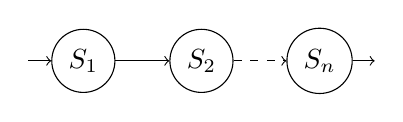
\begin{tikzpicture}
            \node[circle, draw] (s1) at (0,0) {$S_1$};
            \node[circle, draw] (s2) at (1.5,0) {$S_2$};
            \node[circle, draw] (sn) at (3,0) {$S_n$};
            \draw[->] (-0.7,0) -- (s1);
            \draw[->] (s1) -- (s2);
            \draw[dashed, ->] (s2) -- (sn);
            \draw[->] (sn) -- (3.7,0);
        \end{tikzpicture}
        &
        \hspace{0.5cm}
        &
        % Series with multiple outputs
        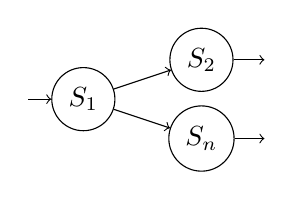
\begin{tikzpicture}
            \node[circle, draw] (s1) at (0,0) {$S_1$};
            \node[circle, draw] (s2) at (1.5,0.5) {$S_2$};
            \node[circle, draw] (sn) at (1.5,-0.5) {$S_n$};
            \draw[->] (-0.7,0) -- (s1);
            \draw[->] (s1) -- (s2);
            \draw[->] (s1) -- (sn);
            \draw[->] (s2) -- (2.3,0.5);
            \draw[->] (sn) -- (2.3,-0.5);
        \end{tikzpicture}
        \\[0.3cm]
        (a) Simple series & & (b) Series with multiple outputs 
        \\[0.5cm]
        % Parallel composition
        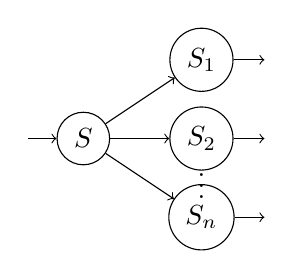
\begin{tikzpicture}
            \node[circle, draw] (s)  at (0,0)   {$S$};
            \node[circle, draw] (s1) at (1.5,1) {$S_1$};
            \node[circle, draw] (s2) at (1.5,0) {$S_2$};
            \node[circle, draw] (sn) at (1.5,-1){$S_n$};
            \draw[->] (-0.7,0) -- (s);
            \draw[->] (s) -- (s1);
            \draw[->] (s) -- (s2);
            \draw[->] (s) -- (sn);
            \draw[->] (s1) -- (2.3,1);
            \draw[->] (s2) -- (2.3,0);
            \draw[->] (sn) -- (2.3,-1);
            \node at (1.5,-0.5) {\vdots};
        \end{tikzpicture}
        &
        \hspace{0.5cm}
        &
        % Negative loop
        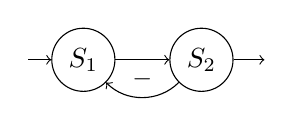
\begin{tikzpicture}
            \node[circle, draw] (s1) at (0,0) {$S_1$};
            \node[circle, draw] (s2) at (1.5,0) {$S_2$};
            \draw[->] (-0.7,0) -- (s1);
            \draw[->] (s1) -- (s2);
            \draw[->] (s2) -- (2.3,0);
            \draw[->, bend left=45] (s2) to 
                node[above]{\small$-$} (s1);
        \end{tikzpicture}
        \\[0.3cm]
        (c) Parallel composition & & (d) Negative loop 
        \\[0.5cm]
        % Inhibition of a behavior
        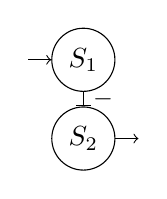
\begin{tikzpicture}
            \node[circle, draw] (s1) at (0,0.5) {$S_1$};
            \node[circle, draw] (s2) at (0,-0.5) {$S_2$};
            \draw[->] (-0.7,0.5) -- (s1);
            \draw[-|] (s1) -- node[right]{\small$-$} (s2);
            \draw[->] (s2) -- (0.7,-0.5);
        \end{tikzpicture}
        &
        \hspace{0.5cm}
        &
        % Contralateral inhibition
        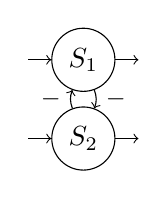
\begin{tikzpicture}
            \node[circle, draw] (s1) at (0,0.5) {$S_1$};
            \node[circle, draw] (s2) at (0,-0.5) {$S_2$};
            \draw[->] (-0.7,0.5) -- (s1);
            \draw[->] (-0.7,-0.5) -- (s2);
            \draw[->, bend left=20] (s1) to 
                node[right]{\small$-$} (s2);
            \draw[->, bend left=20] (s2) to 
                node[left]{\small$-$} (s1);
            \draw[->] (s1) -- (0.7,0.5);
            \draw[->] (s2) -- (0.7,-0.5);
        \end{tikzpicture}
        \\[0.3cm]
        (e) Inhibition of a behavior & & (f) Contralateral inhibition
    \end{tabular}
    \caption{The six fundamental neuronal archetypes, 
    adapted from~\cite{demaria2020formal}.}
    \label{fig:archetypes}
\end{figure}

These archetypes are biologically inspired logical operators, 
easily adjustable by tuning a small number of parameters, and 
they constitute the basis of typical instances of neuronal 
information processing~\cite{demaria2020formal}.

% ---------------------------------------------------------------
\section{Temporal Logic and Model Checking}
\label{sec:modelchecking}

Formal verification of neuronal archetypes requires a rigorous 
framework for expressing and checking properties of the neural 
network over time. This section introduces the three foundational 
steps of the model checking approach used in this work: transition 
systems as the semantic model of computation, temporal logic as 
the language for expressing properties, and model checking as the 
automated verification procedure~\cite{Clarke1999}.

\subsection{Transition Systems}

A transition system is a mathematical structure used to model the
dynamic behavior of a reactive or computational
system~\cite{Clarke1999}. It captures all possible states the system
may occupy and all possible ways the system may evolve from one state
to another in response to inputs or internal events.

Formally, a transition system is a tuple
$\mathcal{T} = (S, S_0, \Sigma, \rightarrow, AP, L)$, where:

\begin{itemize}
    \item $S$ is a finite or infinite set of states,
    \item $S_0 \subseteq S$ is the set of initial states,
    \item $\Sigma$ is a set of actions or inputs,
    \item $\rightarrow\ \subseteq S \times \Sigma \times S$ is the
    transition relation, where $(s, a, s') \in\ \rightarrow$ means
    that the system can move from state $s$ to state $s'$ upon
    action $a$. The transition relation is required to be 
    \emph{global}: for every state $s \in S$, there must exist 
    at least one outgoing transition, ensuring that no execution 
    becomes stuck~\cite{Clarke1999},
    \item $AP$ is a set of atomic propositions describing observable
    properties of states,
    \item $L : S \rightarrow 2^{AP}$ is a labeling function assigning
    to each state the set of atomic propositions that hold in that
    state~\cite{Clarke1999}.
\end{itemize}

An \emph{execution} of a transition system is a (finite or infinite)
sequence of states $s_0, s_1, s_2, \ldots$ such that $s_0 \in S_0$
and $(s_i, a_i, s_{i+1}) \in\ \rightarrow$ for each consecutive pair.
The set of all executions defines the behavior of the
system~\cite{Clarke1999}.

We consider a discretized version of LI\&F networks. In this 
setting, the states of the transition system capture the membrane 
potentials and spike emission statuses of all neurons in the 
network at a given discrete time instant. Each transition encodes 
one time step of the neural computation, during which every neuron 
updates its potential and possibly emits a spike according to the 
LI\&F equations of Definition~\ref{def:lif}. Because the 
integration window $\sigma$ is bounded and weights are rational, 
the resulting state space is finite, which makes the system 
amenable to automatic 
verification~\cite{DeMaria2016,DeMaria2017}.

The integration window $\sigma$ used in the LI\&F model determines
the bound on the state space: given a leak factor $r \in (0,1)$
and an approximation error threshold $\varepsilon > 0$, the
condition $r^e \leq \varepsilon$ gives:
\[
e \cdot \ln(r) \leq \ln(\varepsilon)
\]
Since $\ln(r) < 0$, dividing both sides by $\ln(r)$ reverses the
inequality:
\[
e \geq \frac{\ln(\varepsilon)}{\ln(r)}
\]
The integration window is therefore:
\[
\sigma = \left\lfloor \frac{\ln(\varepsilon)}{\ln(r)}
\right\rfloor
\]
For example, with $r = 0.9$ and $\varepsilon = 0.01$:
\[
\sigma = \left\lfloor \frac{\ln(0.01)}{\ln(0.9)} \right\rfloor
= \left\lfloor \frac{-4.605}{-0.105} \right\rfloor
= \lfloor 43.8 \rfloor = 43 \text{ time steps}
\]
With $r = 0.5$ and $\varepsilon = 0.01$:
\[
\sigma = \left\lfloor \frac{\ln(0.01)}{\ln(0.5)} \right\rfloor
= \left\lfloor \frac{-4.605}{-0.693} \right\rfloor
= \lfloor 6.64 \rfloor = 6 \text{ time steps}
\]
This shows that a smaller leak factor $r$ produces a shorter
effective memory window, which directly reduces the size of the
state space and improves model checking
efficiency~\cite{DeMaria2016,DeMaria2017}.

\subsection{Temporal Logic}

Temporal logic extends classical propositional or first-order logic
with operators that express how the truth of propositions evolves 
over time along the executions of a transition
system~\cite{Clarke1999}. It provides a precise and expressive
language for stating properties such as ``a neuron always eventually
emits a spike'' or ``once the inhibitory signal fires, the target
neuron never emits again.'' Two major families of temporal logic are
used in practice: Computation Tree Logic 
(CTL)~\cite{Clarke1986} and Linear Temporal
Logic (LTL)~\cite{Pnueli1977}.

\subsubsection{Computation Tree Logic (CTL)}

CTL was introduced by Clarke, Emerson, and Sistla as a logic for 
reasoning over the branching-time structure of 
computation~\cite{Clarke1986}. It interprets properties over the 
tree of all possible futures branching from a given state. In CTL, 
every temporal operator is paired with a path quantifier that 
specifies whether the property must hold on \emph{all} paths or on 
\emph{some} (at least one) path from the current state. The two 
path quantifiers are:

\begin{itemize}
    \item $\mathbf{A}$ (for all paths): the property must hold on
    every possible future execution,
    \item $\mathbf{E}$ (there exists a path): the property must hold
    on at least one possible future execution.
\end{itemize}

These quantifiers are combined with temporal operators:

\begin{itemize}
    \item $\mathbf{X}\,\varphi$ (\emph{next}): $\varphi$ holds in
    the next state,
    \item $\mathbf{F}\,\varphi$ (\emph{finally/eventually}):
    $\varphi$ holds at some future state,
    \item $\mathbf{G}\,\varphi$ (\emph{globally/always}): $\varphi$
    holds in every future state,
    \item $\varphi\,\mathbf{U}\,\psi$ (\emph{until}): $\varphi$
    holds continuously until $\psi$ becomes
    true~\cite{Clarke1986,Clarke1999}.
\end{itemize}

A CTL formula always combines exactly one path quantifier with
exactly one temporal operator, yielding expressions of the form
$\mathbf{AX}\,\varphi$, $\mathbf{EF}\,\varphi$,
$\mathbf{AG}\,\varphi$, and so on~\cite{Clarke1986}. For example:

\begin{itemize}
    \item In the Lustre implementation of the LI\&F
    model~\cite{DeMaria2016}, spike emission is delayed by one time
    unit to prevent simultaneous reception and emission. The CTL
    formula expressing this is:
    \[
    \mathbf{AG}(\mathit{p(t) > \tau}
    \Rightarrow \mathbf{AX}\,\mathit{spike})
    \]
    which states that on all paths, whenever a neuron's membrane 
    potential exceeds the threshold $\tau$ at time $t$, a spike 
    will be emitted at time $t + 1$.
    \item $\mathbf{EF}\,\mathit{oscillation}$ states that there
    exists at least one execution on which an oscillating behavior
    is eventually reached~\cite{DeMaria2016,DeMaria2017}.
\end{itemize}

CTL is well suited for expressing properties that depend on the
branching structure of the computation tree, in particular those
involving existential guarantees or conditions that may differ 
across execution paths.

\subsubsection{Linear Temporal Logic (LTL)}

LTL was introduced by Pnueli as a logic for reasoning about the 
temporal behavior of programs along linear execution 
sequences~\cite{Pnueli1977}. An LTL formula is evaluated over a 
single infinite sequence of states $s_0, s_1, s_2, \ldots$ and is
satisfied by the system if it holds on \emph{all} its executions.
LTL uses the same temporal operators ($\mathbf{X}$, $\mathbf{F}$,
$\mathbf{G}$, $\mathbf{U}$) but without explicit path quantifiers,
since the universal quantification over all paths is 
implicit~\cite{Pnueli1977,Clarke1999}.

For example:

\begin{itemize}
    \item $\mathbf{G}(\mathit{input} \Rightarrow
    \mathbf{F}\,\mathit{spike})$ states that every time an input
    is received, a spike is eventually emitted.
    \item $\mathbf{G}\,\neg(\mathit{spike}_1 \wedge
    \mathit{spike}_2)$ expresses that two neurons never fire
    simultaneously --- a mutual exclusion property relevant to the
    series with multiple outputs archetype (Property~3 of
    Section~\ref{sec:modelchecking})~\cite{DeMaria2016,DeMaria2017}.
\end{itemize}

LTL is generally more natural for expressing safety and liveness
properties along individual executions and is the temporal logic
most directly supported by the Lustre observer
mechanism~\cite{Halbwachs1993,Halbwachs1998}.

\subsection{Model Checking}

Model checking is an automated technique for verifying whether a
transition system $\mathcal{T}$ satisfies a temporal logic formula
$\varphi$, written $\mathcal{T} \models \varphi$~\cite{Clarke1999}.
Given a finite-state transition system and a formula expressed in
CTL or LTL, a model checker systematically explores all reachable
states of the system and determines whether the property holds in
every initial state and along every execution path.

The general model checking procedure proceeds as follows. First,
the system under study is encoded as a transition system, either
explicitly as a state graph or symbolically using a compact
representation such as Binary Decision Diagrams
(BDDs)~\cite{Burch1994} or Satisfiability Modulo Theories (SMT)
formulas~\cite{Hagen2008,Champion2016}. Second, the property of
interest is expressed in a temporal logic formalism. Third, the
model checker traverses the state space and checks whether the
formula holds. For CTL model checking, this is done by a labeling
algorithm that annotates each state with the sub-formulas that hold
in it, proceeding inductively from atomic propositions up to the
full formula~\cite{Clarke1999}. For LTL model checking, the
standard approach converts the negation of the formula into a
B\"{u}chi automaton and checks whether the product of this
automaton with the transition system has any accepting run --- if
so, a counterexample is found~\cite{Clarke1999}.

A crucial feature of model checkers is their ability to produce
\emph{counterexamples}: when a property does not hold, the tool
automatically generates an execution trace that witnesses the
violation~\cite{Clarke1999}. This is particularly valuable in the
neuronal archetype context, as a counterexample identifies the
precise sequence of membrane potential updates and spike emissions
that violates the expected behavior, guiding the refinement of
either the model parameters or the property
formulation~\cite{DeMaria2016,DeMaria2017}.

In practice, when the state space is too large for explicit
enumeration, modern model checkers rely on symbolic
methods~\cite{Burch1994,Clarke1994,Clarke1999b}. For instance, 
the Kind2 model checker combines k-induction with SMT 
solving~\cite{Hagen2008,Champion2016}, which allows it to reason
about infinite-horizon properties of reactive systems --- such as
perpetual oscillation in a negative loop --- without explicitly
enumerating all reachable 
states~\cite{DeMaria2016,DeMaria2017}.

In~\cite{DeMaria2016,DeMaria2017} the neuronal archetypes are 
encoded as a Lustre transition system and the property of interest 
is expressed as a Lustre observer node. Kind2 then takes both as 
input and either confirms the property or produces a counterexample 
trace~\cite{Hagen2008,Champion2016}. When the property is refuted, 
the counterexample guides the refinement of model parameters or the 
reformulation of the property before the process is repeated. This 
closed verification loop is the foundation of the model checking 
approach applied throughout 
Section~\ref{sec:modelchecking}~\cite{DeMaria2016,DeMaria2017}.

% ---------------------------------------------------------------
\section{Tools}

To practically evaluate the theoretical framework established in 
the previous sections, dedicated software tools for model checking 
are required. Relevant temporal properties of these models are 
often specified using temporal logic and verified through model 
checking tools such as NuSMV~\cite{Cimatti1999} or 
PRISM~\cite{Kwiatkowska2011}.

For the experimental implementation considered in this work, we 
focus on NuSMV~\cite{Cimatti1999}, a widely used symbolic model 
verifier built on Binary Decision Diagrams (BDDs). NuSMV supports 
verification of finite-state systems against specifications written 
in both Computation Tree Logic (CTL) and Linear Temporal Logic 
(LTL), making it well suited to expressing the temporal firing 
properties of neuronal archetypes. The discrete states, recursive 
membrane potential equations, and threshold-triggered transition 
relations of the LIF neuron model can be mapped directly into 
NuSMV's modular architecture, allowing the reachable state space 
of the network to be systematically explored. When a property does 
not hold, NuSMV automatically produces a counterexample trace that 
identifies the precise sequence of membrane potential updates and 
spike emissions responsible for the violation, guiding further 
refinement of the model or its parameters.

\section{Verification Pipeline for Spiking Neural Network Models}

To practically evaluate the theoretical framework established in the previous sections,
we propose a two-layer automated pipeline designed to support the formal modelling and
verification of Spiking Neural Networks (SNNs). This pipeline enables the transformation
of high-level network descriptions into formally analysable models, which are then verified
using model checking techniques.

\subsection{System Architecture}

The pipeline consists of two main stages. In the first stage, \emph{Model Generation},
a Domain-Specific Language (DSL) is used to describe the structure and dynamics of a
neural network. This high-level specification is compiled into a formal model represented
as a finite-state transition system, encoded in the \texttt{.smv} format compatible with
the NuSMV model checker~\cite{nusmv}. In the second stage, \emph{Model Checking}, the
generated \texttt{.smv} model is executed in NuSMV to verify temporal logic properties
expressed in CTL or LTL. The verification process determines whether these properties
hold and produces detailed outputs for further analysis. This architecture follows the
classical formal verification workflow: system specification $\rightarrow$ model
construction $\rightarrow$ property verification.

\subsection{Compilation from DSL to Formal Model}

The transformation from DSL to a formal model is the core component of the system, as
it directly impacts the correctness and expressiveness of the verification process.

\subsubsection{Neural Network Representation}

The neural network is internally represented as a directed graph in which nodes represent
neurons and input signals, while edges represent synaptic connections, which can be
excitatory or inhibitory. In addition to the graph structure, the system introduces the
concept of \emph{archetypes}, which capture common structural motifs observed in neural
networks, as described in Section~2. These archetypes enable higher-level reasoning about
network behavior beyond individual connections.

\subsubsection{DSL Parsing}

During parsing, the system extracts the set of neurons and input signals, the connectivity
structure of the network, temporal input schedules, user-defined specifications, and
explicit archetype definitions when provided. The result of this step is an intermediate
representation that serves as a bridge between the high-level DSL and the formal model.

\subsubsection{Identifier Sanitization}

A practical challenge in generating NuSMV models is avoiding conflicts with reserved
keywords. To ensure syntactic correctness, all identifiers (e.g., neuron names, input
variables) are automatically sanitized. If a name conflicts with a reserved keyword or
follows a problematic pattern, it is transformed into a safe equivalent, guaranteeing
that the generated model remains valid regardless of the naming choices made in the DSL.

\subsubsection{Automatic Archetype Detection}

When archetypes are not explicitly specified, the system automatically detects them
using structural pattern recognition applied to the graph. The heuristic rules employed
include: mutual inhibitory connections, which signal a negative loop; symmetric inhibition
patterns, which indicate contralateral inhibition; and linear connectivity, which
corresponds to a sequential chain. This capability reduces the burden on users and allows
the system to infer meaningful structural patterns that govern network behavior.

\subsubsection{Automatic Property Generation}

A key feature of the system is the automatic generation of temporal logic properties
based on detected archetypes. For example, in the case of a negative feedback loop, the
system generates properties that capture mutual exclusion (two neurons should not fire
simultaneously), reachability (each neuron can eventually become active), and causality
(activation of one neuron may lead to activation of another in the future). These
properties are expressed in CTL and embedded directly into the model, removing the need
for users to manually define complex temporal specifications.

\subsubsection{NuSMV Model Generation}

After all transformations are complete, the system produces a fully specified
\texttt{.smv} model encoding the following elements. State variables capture the global
time, input signals, and neuron states. Transition rules describe the evolution of
neuron states according to the LIF model defined in Section~2, as well as the evolution
of inputs through predefined schedules or nondeterministic behavior. Verification
properties include baseline properties, composition-related properties, automatically
generated archetype properties, and user-defined specifications. This model constitutes
a finite-state transition system suitable for model checking, consistent with the
framework described in Section~3.

\subsection{End-to-End Execution Workflow}

The entire verification process is orchestrated by an automated wrapper that simplifies
user interaction with the pipeline. When a verification command is executed, the system
proceeds through the following steps: parsing the DSL specification; constructing the
internal graph-based representation; sanitizing all identifiers; detecting archetypes
within the network; generating corresponding verification properties; producing the
\texttt{.smv} model; executing the model in NuSMV; and finally analysing and summarising
the results. The output includes the number of satisfied properties, the number of
violated properties, and detailed logs for debugging and analysis. This automation
eliminates the need for manual interaction with the model checker and allows users to
perform the full verification pipeline through a single command.

```latex
% ============================================================
\section{Architecture and Processing Flow of the \texttt{snn\_mc} System}
\label{sec:snn_mc_pipeline}
% ============================================================

This section presents the \texttt{snn\_mc} system --- a software tool developed to directly implement the formal verification framework introduced in the previous sections. The system takes as input a spiking neural network architecture description file written in a domain-specific language (\textit{domain-specific language}, DSL), automatically generates the corresponding NuSMV code for the discrete LIF model together with temporal specifications (CTLSPEC/LTLSPEC), then invokes NuSMV for verification and result summarization. This entire workflow directly reflects the theoretical process described in~\cite{demaria2020formal,DeMaria2016,DeMaria2017}, while being fully automated and integrated into a complete pipeline.

\subsection{System Overview}

The \texttt{snn\_mc} system is designed following a linear pipeline architecture, where each stage receives the output of the previous stage and produces a higher-level intermediate representation. All orchestration logic is centralized in the \texttt{main()} function inside the file \texttt{snn\_mc/cli.py}, which serves as the unique entry point and controller of the system. The remaining modules do not execute any tasks when loaded into memory; they are only invoked by this orchestration layer or by the testing framework. This design ensures simplicity of the execution flow and facilitates independent testing of each component.

Users interact with the system through a command-line interface using the following syntax:

\begin{lstlisting}
python -m snn_mc run examples/series_negloop.dsl --out runs/demo
\end{lstlisting}

The above command activates the processing chain from the network description file in \texttt{.dsl} format to the set of output files including NuSMV code, verification logs, and demonstration reports.

\subsection{End-to-End Verification Pipeline}

Figure~\ref{fig:pipeline_flow} illustrates the complete processing workflow of the system, from the input \texttt{.dsl} file to the collection of output artefacts written on disk. Each processing stage corresponds to one step of the formal verification workflow: parsing, constraint checking, representation preparation, code generation, verification, and result summarization.

% Add this package in the preamble if it is not already included:
% \usepackage{graphicx}

\begin{figure}[H]
\vspace{-0.4cm}
\centering
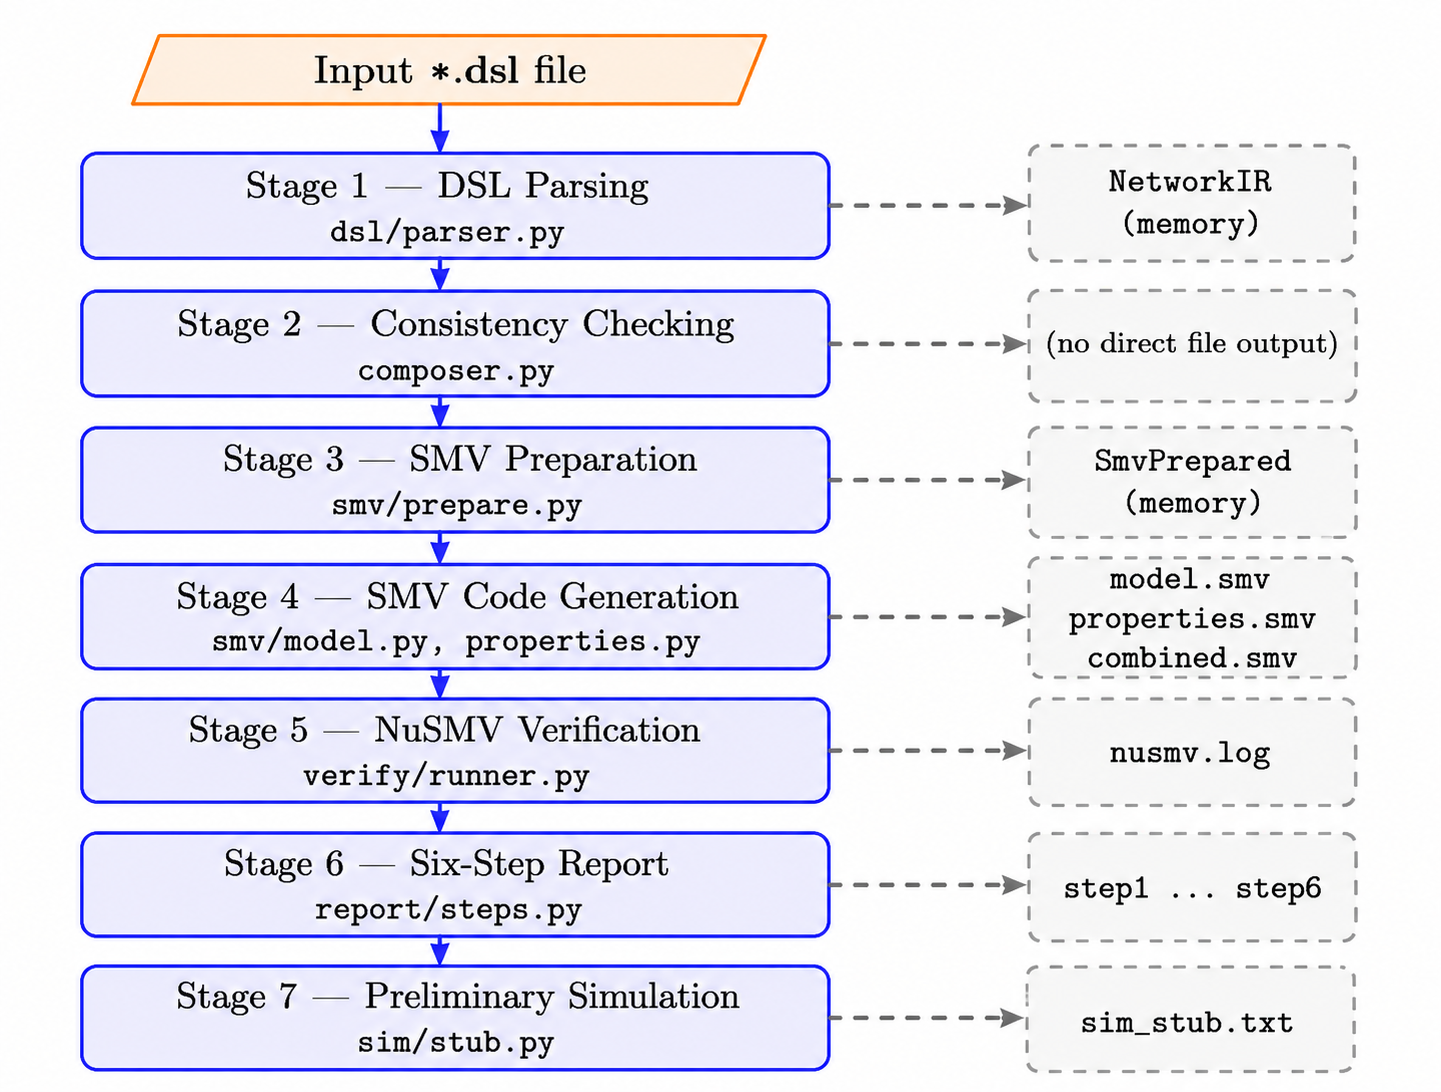
\includegraphics[width=0.92\linewidth]{pipeline_flowchart.png}
\vspace{-0.3cm}
\caption{Processing workflow of the \texttt{snn\_mc} system: from the input DSL file to the output artefacts. Solid arrows represent the main control flow; dashed arrows represent intermediate artefacts or output files written to disk.}
\vspace{-0.5cm}
\label{fig:pipeline_flow}
\end{figure}

\paragraph{DSL Parsing and Intermediate Representation.}

The starting point of the pipeline is the \texttt{parse\_file()} function in the module \texttt{snn\_mc/dsl/parser.py}. This function reads the \texttt{.dsl} file, processes \texttt{include} directives through \texttt{expand\_includes()} in order to flatten imported files, then forwards the entire source text to the functions \texttt{parse\_text()} and \texttt{\_parse\_body()} for semantic line-by-line analysis.

The result of this stage is a \texttt{NetworkIR} object --- an intermediate data structure storing all network information in memory. This structure includes the set of neurons, the set of directed edges (\texttt{Edge}) with excitatory or inhibitory weights corresponding to the weighted graph definition introduced in Section~2.2, archetype instances (\texttt{ArchetypeInstance}), LIF parameters (\texttt{ParamSpec}) representing the triplet $(\tau, r, w_i)$ introduced in Section~2.4, and composition declarations (\texttt{Composition}).

A dedicated mechanism is implemented to handle block declarations (\texttt{block}): when the parser encounters the command \texttt{block simple\_series input=stim N=4 prefix=c}, it queries the architecture registry \texttt{BLOCK\_REGISTRY}, then invokes the \texttt{apply\_block()} method of the corresponding architecture class. This method automatically generates neuron names (\texttt{c1}, \texttt{c2}, \ldots, \texttt{cN}) and inserts \texttt{Edge} objects into \texttt{NetworkIR}, enabling complex network structures such as the archetypes introduced in Section~2.5 to be described using only a concise single-line declaration.

\paragraph{Consistency Checking and Composition Validation.}

After DSL parsing, the \texttt{NetworkIR} object is passed to the \texttt{compose()} function in \texttt{snn\_mc/composer.py}. This stage does not modify the network topology but only performs reference consistency checking: every \texttt{input=} declaration inside a block must point either to a declared input or to an already existing neuron in \texttt{ir.neurons}. For example, if the \texttt{negative\_loop} block declares \texttt{input=c4}, then neuron \texttt{c4} must already have been generated by the preceding \texttt{simple\_series} block. If the constraint is violated, the system immediately raises a \texttt{ValueError}, detecting the error before NuSMV code generation and avoiding difficult-to-trace issues during the verification stage.

\paragraph{SMV Representation Preparation.}

The \texttt{prepare\_ir()} function in \texttt{snn\_mc/smv/prepare.py} transforms \texttt{NetworkIR} into a \texttt{SmvPrepared} structure --- an immutable snapshot shared by all downstream code generation modules. This process consists of three main steps.

First, identifiers are normalized into a valid NuSMV format through \texttt{sanitize\_identifier()}, removing special characters not accepted by the verifier. Next, edges are grouped according to their effect direction: each neuron receives a separate list of excitatory sources (\texttt{exc\_srcs}) and inhibitory sources (\texttt{inh\_srcs}), directly reflecting the spatial summation mechanism described in Section~2.1. Finally, the system merges explicitly declared archetypes with automatically detected architectures obtained through graph analysis (\texttt{detect\_archetypes}), enriching the representation with architectural semantics for unnamed structural patterns.

\paragraph{NuSMV Code Generation.}

The SMV code generation layer consists of four specialized modules, all receiving \texttt{SmvPrepared} as input and generating the corresponding NuSMV text. The module \texttt{smv/model.py} generates the body of the main program (\texttt{MODULE main}) with variable declarations, assignments, and neuron instances. The module \texttt{smv/lif\_module.py} generates the LIF module definition describing membrane dynamics with membrane potential~$p(t)$, leak constant~$r$, and firing threshold~$\tau$ --- this is a direct implementation of the recursive equation defined in Section~2.3. The module \texttt{smv/properties.py} generates verification specifications in the form of CTLSPEC and LTLSPEC as presented in Section~3.2, while \texttt{smv/combined.py} merges everything into a single \texttt{combined.smv} file.

The system supports two neuron encoding modes through the \texttt{--emit-mode} parameter: the default \texttt{lif} mode uses the complete representation with continuous membrane potential variables, while the \texttt{simple\_boolean} mode uses a discrete threshold representation similar to the McCulloch--Pitts model to reduce state-space complexity when necessary.

\paragraph{Formal Verification and Result Analysis.}

The verification stage is implemented by two modules in the \texttt{verify/} directory, corresponding to the NuSMV tool introduced in Section~4. The function \texttt{run\_nusmv()} in \texttt{verify/runner.py} locates the NuSMV executable on the system, then launches NuSMV as a subprocess using the \texttt{combined.smv} file as input and writes the log to \texttt{nusmv.log}. The function \texttt{summarize\_nusmv\_output()} in \texttt{verify/result.py} analyzes this log, counts the number of satisfied (\texttt{is true}) and violated (\texttt{is false}) specifications, and extracts counterexample traces (\textit{counterexample}) through \texttt{extract\_counterexample\_block()} whenever a specification is not satisfied. This counterexample mechanism directly supports the model parameter refinement objective discussed in Section~3.3. This stage can be skipped using the \texttt{--skip-verify} flag.

\paragraph{Six-Step Report Generation.}

The function \texttt{write\_all\_steps()} in \texttt{snn\_mc/report/steps.py} is always executed regardless of the verification result, generating six files intended for demonstration and intermediate inspection purposes. Each file corresponds to one conceptual stage in the analysis workflow: \texttt{step1\_diagram.md} presents the network diagram in Mermaid and ASCII formats generated from \texttt{NetworkIR.edges}; \texttt{step2\_input.dsl} is a verbatim copy of the original input file; \texttt{step3\_ir.json} contains the JSON representation of \texttt{NetworkIR} for internal inspection; \texttt{step4\_composition.txt} describes the list of architectures and compositions extracted from \texttt{SmvPrepared}; \texttt{step5\_properties.smv} lists the formal specifications; and \texttt{step6\_results.txt} summarizes the verification results together with counterexamples if any.

\paragraph{Simulation Support.}

The final stage in the pipeline is the \texttt{run\_simulation\_stub()} function in \texttt{snn\_mc/sim/stub.py}. This stage is only activated when three conditions are simultaneously satisfied: the \texttt{--skip-sim} flag is not set, the verification stage has been executed, and all specifications return \texttt{true}. Instead of performing a complete LIF simulation --- which is unnecessary because NuSMV already serves as the authority regarding model correctness --- this module generates the \texttt{sim\_stub.txt} file containing a wiring summary of excitatory and inhibitory inputs for each neuron, helping users inspect the network configuration at a high level without reading SMV code.

\subsection{Archetype Mechanism}

One of the most notable design features of \texttt{snn\_mc} is its archetype mechanism, which directly implements the six theoretical archetypes presented in Section~2.5. The system registers seven block types in the directory \texttt{snn\_mc/archetypes/}: simple series (\texttt{simple\_series}), multiple-output series (\texttt{series\_multiple\_outputs}), parallel composition (\texttt{parallel\_composition}), negative feedback loop (\texttt{negative\_loop}), positive feedback loop (\texttt{positive\_loop}), contralateral inhibition (\texttt{contralateral\_inhibition}), and inhibition of behavior (\texttt{inhibition\_of\_behavior}). Compared with the six theoretical archetypes, the system introduces the \texttt{positive\_loop} architecture as a practical extension.

Each archetype class inherits from \texttt{archetypes/base.py} and implements two main methods: \texttt{apply\_block()}, responsible for generating the corresponding neurons and edges; and \texttt{specs()}, responsible for generating CTLSPEC/LTLSPEC specifications characteristic of that architecture according to the properties defined in~\cite{demaria2020,demaria2016}. The utility function \texttt{expand\_chain()} in the base class handles automatic name generation according to the \texttt{prefix\{1..N\}} rule, while \texttt{stim\_token()} converts input references into the appropriate LTL syntax when \texttt{input=} points to a neuron (\texttt{c4.spike}) instead of a system input.

\subsection{Project Organization and Exit Codes}

The entire source code of the system is organized under the directory \texttt{NewStructure/snn\_mc/} with six functional subdirectories: \texttt{dsl/} converts DSL text into \texttt{NetworkIR}; \texttt{archetypes/} defines network block types; \texttt{smv/} translates IR into NuSMV source code; \texttt{verify/} invokes NuSMV and analyzes logs; \texttt{sim/} generates post-verification wiring summaries; and \texttt{report/} exports the six demonstration files. The system returns meaningful exit codes: 0 for success or skipped verification; 1 when at least one specification fails; 2 when the DSL file cannot be found; 3 when NuSMV is not available in the \texttt{PATH}; and 4 when the log contains no \texttt{is true} line, which usually indicates an SMV syntax error.
```


% ---------------------------------------------------------------
\begin{thebibliography}{99}

\bibitem{Thomas1995}
Thomas, R., Thieffry, D., Kaufman, M.: Dynamical behaviour of
biological regulatory networks --- I. Biological role of feedback
loops and practical use of the concept of the loop-characteristic
state. Bulletin of Mathematical Biology \textbf{57}(2), 247--276
(1995).
\doi{10.1007/BF02460618}

\bibitem{Reddy1993}
Reddy, V.N., Mavrovouniotis, M.L., Liebman, M.N.: Petri net
representations in metabolic pathways. In: Proceedings of the 1st
International Conference on Intelligent Systems for Molecular
Biology, pp. 328--336. AAAI Press (1993)

\bibitem{Regev2001}
Regev, A., Silverman, W., Shapiro, E.: Representation and simulation
of biochemical processes using the $\pi$-calculus process algebra.
In: Proceedings of the 6th Pacific Symposium on Biocomputing,
pp. 459--470 (2001)

\bibitem{Regev2004}
Regev, A., Panina, E.M., Silverman, W., Cardelli, L., Shapiro, E.:
BioAmbients: an abstraction for biological compartments. Theoretical
Computer Science \textbf{325}(1), 141--167 (2004).
\doi{10.1016/j.tcs.2004.03.065}

\bibitem{Chabrier2004}
Chabrier-Rivier, N., Chiaverini, M., Danos, V., Fages, F.,
Sch\"{a}chter, V.: Modeling and querying biomolecular interaction
networks. Theoretical Computer Science \textbf{325}(1), 25--44
(2004).
\doi{10.1016/j.tcs.2004.03.063}

\bibitem{Hofestädt1998}
Hofest\"{a}dt, R., Thelen, S.: Quantitative modeling of biochemical
networks. In Silico Biology \textbf{1}, 39--53 (1998)

\bibitem{Alur2001}
Alur, R., Belta, C., Ivancic, F.: Hybrid modeling and simulation of
biomolecular networks. In: Hybrid Systems: Computation and Control,
HSCC 2001, pp. 19--32. Springer (2001).
\doi{10.1007/3-540-45351-2\_6}

\bibitem{Phillips2007}
Phillips, A., Cardelli, L.: Efficient, correct simulation of
biological processes in the stochastic $\pi$-calculus. In:
Computational Methods in Systems Biology, CMSB 2007, pp. 184--199.
Springer (2007).
\doi{10.1007/978-3-540-75140-3\_13}

\bibitem{Danos2004}
Danos, V., Laneve, C.: Formal molecular biology. Theoretical
Computer Science \textbf{325}(1), 69--110 (2004).
\doi{10.1016/j.tcs.2004.03.065}

\bibitem{Cimatti1999}
Cimatti, A., Clarke, E.M., Giunchiglia, F., Roveri, M.: NuSMV: a
new symbolic model verifier. In: Computer Aided Verification,
CAV 1999, pp. 495--499. Springer (1999).
\doi{10.1007/3-540-48683-6\_44}

\bibitem{Kwiatkowska2011}
Kwiatkowska, M.Z., Norman, G., Parker, D.: PRISM 4.0: verification
of probabilistic real-time systems. In: Computer Aided Verification,
CAV 2011, pp. 585--591. Springer (2011).
\doi{10.1007/978-3-642-22110-1\_47}

\bibitem{demaria2020formal}
De~Maria, E., Bahrami, A., L'Yvonnet, T., Felty, A., Gaff\'{e}, D.,
Ressouche, A., Grammont, F.: On the use of formal methods to model
and verify neuronal archetypes. Frontiers of Computer Science
(2020).
\doi{10.1007/s11704-020-9253-z}

\bibitem{Maass1997}
Maass, W.: Networks of spiking neurons: the third generation of
neural network models. Neural Networks \textbf{10}(9), 1659--1671
(1997).
\doi{10.1016/S0893-6080(97)00011-7}

\bibitem{McCulloch1943}
McCulloch, W.S., Pitts, W.: A logical calculus of the ideas
immanent in nervous activity. Bulletin of Mathematical Biophysics
\textbf{5}(4), 115--133 (1943).
\doi{10.1007/BF02478259}

\bibitem{Cybenko1989}
Cybenko, G.: Approximation by superpositions of a sigmoidal
function. Mathematics of Control, Signals and Systems \textbf{2}(4),
303--314 (1989).
\doi{10.1007/BF02551274}

\bibitem{PaugamMoisy2012}
Paugam-Moisy, H., Bohte, S.M.: Computing with spiking neuron
networks. In: Handbook of Natural Computing, pp. 335--376.
Springer (2012).
\doi{10.1007/978-3-540-92910-9\_10}

\bibitem{Hodgkin1952}
Hodgkin, A.L., Huxley, A.F.: A quantitative description of membrane
current and its application to conduction and excitation in nerve.
The Journal of Physiology \textbf{117}(4), 500--544 (1952).
\doi{10.1113/jphysiol.1952.sp004764}

\bibitem{Lapicque1907}
Lapicque, L.: Recherches quantitatives sur l'excitation
\'{e}lectrique des nerfs trait\'{e}e comme une polarisation. Journal
de Physiologie et de Pathologie G\'{e}n\'{e}rale \textbf{9},
620--635 (1907)

\bibitem{Gerstner2002}
Gerstner, W., Kistler, W.: Spiking Neuron Models: An Introduction.
Cambridge University Press, New York (2002)

\bibitem{Aman2016}
Aman, B., Ciobanu, G.: Modelling and verification of weighted
spiking neural systems. Theoretical Computer Science \textbf{623},
92--102 (2016).
\doi{10.1016/j.tcs.2016.01.027}

\bibitem{DeMaria2018}
De~Maria, E., Di~Giusto, C.: Parameter learning for spiking neural
networks modelled as timed automata. In: Proceedings of the 11th
International Joint Conference on Biomedical Engineering Systems
and Technologies, BIOINFORMATICS, pp. 17--28 (2018).
\doi{10.5220/0006540500170028}

\bibitem{yao2023probabilistic}
Yao, X., De~Maria, E., De~Simone, R.: Formal methods for
probabilistic spiking neural networks. In: Proceedings of the
International Conference on Formal Methods for the Design of
Computer, Communication and Software Systems, pp. XX--XX (2023)

\bibitem{Clarke1999}
Clarke, E.M., Grumberg, O., Peled, D.A.: Model Checking. MIT Press,
Cambridge, MA, USA (1999)

\bibitem{Clarke1986}
Clarke, E.M., Emerson, E.A., Sistla, A.P.: Automatic verification
of finite-state concurrent systems using temporal logic
specifications. ACM Transactions on Programming Languages and
Systems \textbf{8}(2), 244--263 (1986).
\doi{10.1145/5397.5399}

\bibitem{Pnueli1977}
Pnueli, A.: The temporal logic of programs. In: Proceedings of
the 18th Annual Symposium on Foundations of Computer Science,
FOCS 1977, pp. 46--57. IEEE (1977).
\doi{10.1109/SFCS.1977.32}

\bibitem{Burch1994}
Burch, J.R., Clarke, E.M., Long, D.E., McMillan, K.L., Dill, D.L.:
Symbolic model checking for sequential circuit verification. IEEE
Transactions on Computer-Aided Design of Integrated Circuits and
Systems \textbf{13}(4), 401--424 (1994).
\doi{10.1109/43.275352}

\bibitem{Clarke1994}
Clarke, E.M., Grumberg, O., Long, D.E.: Model checking and
abstraction. ACM Trans. Program. Lang. Syst. \textbf{16}(5),
1512--1542 (1994).
\doi{10.1145/186025.186051}

\bibitem{Clarke1999b}
Clarke, E.M., Long, D.E., McMillan, K.L.: Compositional model
checking. MIT Press (1999)

\bibitem{Halbwachs1998}
Halbwachs, N.: Synchronous programming of reactive systems. In:
Computer Aided Verification, CAV '98. Lecture Notes in Computer
Science, vol. 1427, pp. 1--16. Springer (1998).
\doi{10.1007/BFb0028727}

\bibitem{Halbwachs1993}
Halbwachs, N., Lagnier, F., Raymond, P.: Synchronous observers and
the verification of reactive systems. In: Third Int. Conf. on
Algebraic Methodology and Software Technology, AMAST'93. Springer
Verlag (1993).
\doi{10.1007/978-1-4471-3227-1\_26}

\bibitem{Hagen2008}
Hagen, G., Tinelli, C.: Scaling up the formal verification of
Lustre programs with SMT-based techniques. In: Formal Methods in
Computer-Aided Design, pp. 1--9 (2008).
\doi{10.1109/FMCAD.2008.ECP.19}

\bibitem{Champion2016}
Champion, A., Mebsout, A., Sticksel, C., Tinelli, C.: The Kind 2
model checker. In: Computer Aided Verification, CAV 2016,
pp. 510--517 (2016).
\doi{10.1007/978-3-319-41540-6\_29}

\bibitem{DeMaria2016}
De~Maria, E., Muzy, A., Gaff\'{e}, D., Ressouche, A., Grammont, F.:
Verification of temporal properties of neuronal archetypes modeled
as synchronous reactive systems. In: Hybrid Systems Biology,
HSB 2016, pp. 97--112 (2016).
\doi{10.1007/978-3-319-47151-8\_7}

\bibitem{DeMaria2017}
De~Maria, E., L'Yvonnet, T., Gaff\'{e}, D., Ressouche, A.,
Grammont, F.: Modelling and formal verification of neuronal
archetypes coupling. In: Proceedings of the 8th International
Conference on Computational Systems-Biology and Bioinformatics,
pp. 3--10 (2017).
\doi{10.1145/3155556.3155557}

\bibitem{Purves2006}
Purves, D., Augustine, G.J., Fitzpatrick, D., Hall, W.C.,
LaMantia, A.S., McNamara, J.O., Williams, S.M. (eds.):
Neuroscience, 3rd edn. Sinauer Associates (2006)

\end{thebibliography}
\end{document}

